% Oral lesion screening under a change of site.
% Compiles with pdfLaTeX + BibTeX (Overleaf: upload this folder, set main.tex as the main file).
% To submit to TMLR: copy the body into the official TMLR Overleaf template and remove the
% author block for the anonymous submission (see README.md in this folder).
\documentclass[11pt]{article}

\usepackage[utf8]{inputenc}
\usepackage[T1]{fontenc}
\usepackage{lmodern}
\usepackage[a4paper,margin=1in]{geometry}
\usepackage{amsmath,amssymb}
\usepackage{graphicx}
\usepackage{booktabs}
\usepackage{multirow}
\usepackage[authoryear,round]{natbib}
\usepackage[hidelinks]{hyperref}
\usepackage{xcolor}
\usepackage{caption}
\captionsetup{font=small,labelfont=bf}

\title{Oral lesion screening from phone photos does not survive a change of site:\\a cross-dataset study of ranking, thresholds and conformal refusal}

\author{Sachchidananda Behera\\
Independent researcher, Bhubaneswar, India\\
\texttt{sachchidananda13@gmail.com}}

\date{}

\begin{document}
\maketitle

\begin{abstract}
Models that flag oral potentially malignant disorders and oral cancer from smartphone photographs report high accuracy, but almost always on photographs from the same source as their training data. We train on one public oral photograph dataset and test on three others, using two model families: a logistic regression on frozen DINOv2 features and an end-to-end fine-tuned ResNet-50. Across countries, the area under the ROC curve falls by up to 0.21, but the operating point fails far more: a model trained on a Chinese dataset clears 97\% of healthy mouths at home and 34\% in an Indian dataset. A split conformal rule that promises 90\% coverage delivers 7\% to 67\% after such a move while still answering most photographs. Fifty labelled photographs from the new site restore the coverage guarantee, but the recalibrated rule then abstains on most of them. A linear classifier separates healthy photographs by dataset with 91\% to 99\% balanced accuracy, and the datasets differ in their share of lesions from 0.2\% to 79\%, which together offer a likely shortcut. Fine-tuning helps in-site and hurts across countries; training on both sites with colour augmentation gave the best results at unseen sites. Between two datasets from one research network and one photo protocol, nothing was lost. We also report that two pairs of these public datasets share photographs, in one case with conflicting labels. Code, splits and all predictions are released.
\end{abstract}

\section{Introduction}

Oral cancer caused an estimated 389{,}000 new cases and 188{,}000 deaths worldwide in 2022, with the largest share in South and South-East Asia \citep{bray2024globocan}. Many cases are found late although early lesions are visible in the mouth, which has led several groups to train image classifiers on photographs taken with ordinary phones, often by community health workers \citep{talwar2023smartphone, piyarathne2024dataset, yu2026opmd}. Reported accuracies are often above 90\%.

Those numbers come from test sets drawn from the same collection as the training set. A screening tool, however, is used somewhere else: by different workers, with different phones and lighting, on a population with a different mix of disease. Radiology has shown that a model can perform well in-site by learning features of the hospital rather than of the disease \citep{zech2018variable, degrave2021shortcuts}, and that such shortcuts are general to deep learning \citep{geirhos2020shortcut}. As far as we can tell, no study has tested oral lesion classifiers across independently collected public datasets.

This paper asks three questions. How much does a classifier lose when moved between public oral photograph datasets? Which part of its behaviour fails: the ranking of photographs, the decision threshold, or a statistical promise to abstain when unsure? And why? We make the following contributions.

\begin{enumerate}
\item A cross-dataset evaluation of two model families on four public datasets from India and China, with patient-level splits, three seeds and patient-level bootstrap intervals. Ranking (AUROC) survives a move much better than the operating point does.
\item A test of split conformal prediction under this shift. The 90\% coverage promise fails badly at a new site, and recalibrating on local photographs restores it at the price of abstaining on most of them.
\item Evidence for a mechanism: healthy photographs carry a dataset signature that a linear model can read, and the datasets differ by two orders of magnitude in how many lesions they contain.
\item An audit of the datasets, which found shared photographs between two pairs, in one case with contradictory labels.
\end{enumerate}

\section{Related work}

\paragraph{Oral lesion classification from photographs.} \citet{talwar2023smartphone} compared deep networks on 2{,}178 smartphone photographs from community screening camps in India. \citet{piyarathne2024dataset} released 3{,}000 annotated phone photographs from Sri Lanka, and \citet{yu2026opmd} compared single- and two-stage classifiers on 1{,}348 photographs from China. These studies evaluate within one collection.

\paragraph{Distribution shift in medical imaging.} \citet{zech2018variable} found that a pneumonia detector trained at one hospital system degraded at others and could identify the hospital from the image. \citet{degrave2021shortcuts} showed COVID-19 detectors relying on markers of the data source. Benchmarks such as WILDS collect real shifts across hospitals \citep{koh2021wilds}, and \citet{gulrajani2021lost} found that many domain generalisation methods do not beat careful empirical risk minimisation. Domain-adversarial training removes features that predict the domain \citep{ganin2016dann}; we do not apply it here but discuss it in Section~\ref{sec:discussion}.

\paragraph{Calibration and conformal prediction.} Modern networks are often miscalibrated even in-site \citep{guo2017calibration}. Split conformal prediction gives a finite-sample coverage guarantee when calibration and test data are exchangeable \citep{vovk2005algorithmic, angelopoulos2021gentle}. Under covariate shift the guarantee needs reweighting \citep{tibshirani2019covariate}, and class-conditional variants guarantee coverage per class \citep{sadinle2019least}. We measure what the plain guarantee delivers when its assumption is broken in the way a deployment would break it.

\section{Data}
\label{sec:data}

We used four public datasets of mouth photographs (Table~\ref{tab:data}). Every class was mapped to the decision a screener makes: \emph{refer} (a potentially malignant disorder or cancer) or \emph{do not refer} (healthy mucosa, a normal variation, or a benign lesion).

\begin{table}[t]
\centering
\caption{Datasets after cleaning. Refer photographs are potentially malignant disorders or cancer. Groups are patients, or clusters of near-identical photographs where no patient id is given.}
\label{tab:data}
\small
\begin{tabular}{llllrrr}
\toprule
Dataset & Country & Source & Role & Photos & Refer & Groups \\
\midrule
SMART-OM & India & \citet{smartom2026} & train, test & 2{,}469 & 145 (5.9\%) & 331 \\
China & China & \citet{yu2026opmd} & train, test & 1{,}348 & 1{,}062 (78.8\%) & 1{,}307 \\
CODE & India & \citet{code2026} & test & 5{,}567 & 13 (0.2\%) & 697 \\
Karnataka & India & \citet{karnataka2021} & test & 313 & 148 (47.3\%) & 313 \\
\bottomrule
\end{tabular}
\end{table}

\paragraph{Cleaning.} SMART-OM and CODE include copies of each photograph with the lesion outline drawn on it; only the unmarked copies were used. CODE version 5 contains 5{,}431 healthy, 166 normal-variation, 14 potentially malignant and 7 cancer photographs, so it serves as a test set only, mainly of false alarms at an unseen centre. Karnataka ships flipped and rotated copies of its photographs, which were excluded.

\paragraph{Shared photographs.} Each photograph was given a 64-bit difference hash, and photographs within 4 bits of each other were treated as the same picture. Ten photographs are identical (0 bits apart) in the China and Karnataka datasets; China labels them leukoplakia or lichen planus and Karnataka labels them malignant. They were removed from Karnataka. SMART-OM and CODE share 33 photographs, including all 7 of CODE's cancer photographs, at distance 0 under different file names. Twenty-five of the 33 pairs are 3 or 4 bits apart and may be different photographs that look alike under a common protocol; all 33 were removed from CODE. No patient identifier appears in both SMART-OM and CODE.

\paragraph{Splits.} SMART-OM and China were split 70/15/15 into train, validation and test by group, stratified by whether a group contains any refer photograph, with three seeds giving three different splits. Where a dataset gives no patient id (China, Karnataka and a small number of SMART-OM files), near-identical photographs were grouped by hash and kept together. CODE and Karnataka are used only for testing. The seed-0 SMART-OM test split holds 358 photographs with 20 refer cases.

\section{Methods}

\paragraph{Models.} The first model is a logistic regression on frozen 768-dimensional features from DINOv2 ViT-B/14 \citep{oquab2023dinov2}, with inputs resized to 224 pixels, features standardised, balanced class weights, and the inverse regularisation strength chosen from $\{0.01, 0.1, 1, 10\}$ by validation AUROC. The second is a ResNet-50 \citep{he2016resnet} initialised from the timm \texttt{a1\_in1k} weights \citep{wightman2021resnet} and fine-tuned end to end for 15 epochs with AdamW (learning rate $10^{-4}$, weight decay $10^{-4}$, batch size 32), a positively weighted binary cross-entropy loss, random resized crops (scale 0.7 to 1.0) and horizontal flips; the epoch with the best validation AUROC is kept. A third variant adds colour jitter (brightness, contrast and saturation 0.4, hue 0.05) and random greyscale ($p=0.1$). ResNet models were trained on copies of each photograph resized to 320 pixels on the long side, to fit a free GPU session. Hyperparameters were fixed in advance and not tuned per site.

\paragraph{Training sites.} Each model was trained on SMART-OM alone and on China alone. The probe and the colour-augmented ResNet were also trained on both together.

\paragraph{Operating point.} The threshold is the highest score that still classifies 90\% of refer photographs correctly on the \emph{training} site's validation split. It is then carried unchanged to every test site. No test-site label is used to choose any parameter, except in the recalibration experiment where that is the point.

\paragraph{Metrics.} We report AUROC, sensitivity and specificity at the carried threshold, and expected calibration error with ten equal-width bins. For each seed, 95\% intervals come from 1{,}000 bootstrap resamples of groups rather than photographs; we report the mean over seeds of the point estimate and of each interval end.

\paragraph{Conformal refusal.} With score $s(x, y) = 1 - \hat p(y \mid x)$, the split conformal quantile $\hat q$ is computed on the training site's validation split at level $\lceil (n+1)(1-\alpha) \rceil / n$ with $\alpha = 0.1$, and the prediction set is $\{y : s(x, y) \le \hat q\}$ \citep{angelopoulos2021gentle}. The model \emph{answers} when the set holds exactly one class and otherwise returns ``not sure, refer''. We report coverage (the true class is in the set) and the share of photographs answered. To recalibrate, $\hat q$ is recomputed from 25, 50 or 100 labelled test-site photographs drawn by group (20 draws per size), which are then excluded from scoring.

\paragraph{Site signature.} For each pair of datasets, a logistic regression on frozen DINOv2 features was trained to predict which dataset a \emph{healthy} photograph came from, so that lesions cannot give the answer away. We report balanced accuracy from five-fold cross-validation with groups kept whole within a fold.

\section{Results}

\subsection{Ranking survives a move; the threshold does not}

Table~\ref{tab:matrix} and Figure~\ref{fig:matrix} give results for every pair of training and test site. Between the two countries AUROC falls by up to 0.21. The operating point fails much more. The China-trained probe clears 97\% of healthy mouths in China and 34\% in SMART-OM, because its mean score for healthy SMART-OM photographs is 0.84 against 0.11 at home. In the other direction, the SMART-OM-trained probe catches 83\% of refer photographs at home and 57\% in China, where its mean score for lesions is 0.34 against 0.61 at home. Expected calibration error rises from 0.03 to 0.79.

\begin{table}[t]
\centering
\caption{Train on one site, test on every site. AUROC with 95\% patient-level bootstrap interval; sensitivity and specificity at the threshold set on the training site; expected calibration error (ECE). Means over three seeds. Diagonal cells are in-site.}
\label{tab:matrix}
\footnotesize
\setlength{\tabcolsep}{4pt}
\begin{tabular}{lllllll}
\toprule
Model & Train & Test & AUROC & Sensitivity & Specificity & ECE \\
\midrule
\multirow{8}{*}{DINOv2 probe}
 & SMART-OM & SMART-OM & 0.90 (0.82--0.96) & 0.83 (0.67--0.95) & 0.83 (0.80--0.87) & 0.08 \\
 & SMART-OM & CODE & 0.89 (0.81--0.96) & 0.82 (0.67--1.00) & 0.78 (0.77--0.79) & 0.13 \\
 & SMART-OM & China & 0.87 (0.81--0.93) & 0.57 (0.49--0.64) & 0.90 (0.80--0.98) & 0.51 \\
 & SMART-OM & Karnataka & 0.80 (0.75--0.85) & 0.82 (0.76--0.88) & 0.62 (0.55--0.69) & 0.13 \\
 & China & China & 0.99 (0.98--1.00) & 0.91 (0.86--0.95) & 0.97 (0.92--1.00) & 0.03 \\
 & China & SMART-OM & 0.83 (0.74--0.90) & 0.97 (0.92--1.00) & 0.34 (0.28--0.39) & 0.79 \\
 & China & CODE & 0.84 (0.67--0.92) & 1.00 (1.00--1.00) & 0.35 (0.33--0.36) & 0.84 \\
 & China & Karnataka & 0.81 (0.77--0.86) & 0.95 (0.91--0.98) & 0.40 (0.33--0.48) & 0.39 \\
\midrule
\multirow{8}{*}{ResNet-50}
 & SMART-OM & SMART-OM & 0.92 (0.85--0.97) & 0.86 (0.70--0.97) & 0.84 (0.79--0.89) & 0.10 \\
 & SMART-OM & CODE & 0.92 (0.85--0.96) & 0.85 (0.58--1.00) & 0.78 (0.77--0.79) & 0.15 \\
 & SMART-OM & China & 0.78 (0.69--0.85) & 0.51 (0.44--0.59) & 0.80 (0.68--0.91) & 0.53 \\
 & SMART-OM & Karnataka & 0.79 (0.73--0.83) & 0.82 (0.76--0.87) & 0.59 (0.51--0.66) & 0.14 \\
 & China & China & 0.98 (0.95--1.00) & 0.94 (0.90--0.97) & 0.94 (0.86--0.99) & 0.05 \\
 & China & SMART-OM & 0.77 (0.69--0.87) & 0.97 (0.90--1.00) & 0.38 (0.31--0.45) & 0.63 \\
 & China & CODE & 0.85 (0.56--0.94) & 0.90 (0.57--1.00) & 0.43 (0.42--0.45) & 0.63 \\
 & China & Karnataka & 0.83 (0.78--0.87) & 0.95 (0.91--0.98) & 0.49 (0.41--0.56) & 0.28 \\
\bottomrule
\end{tabular}
\end{table}

\begin{figure}[t]
\centering
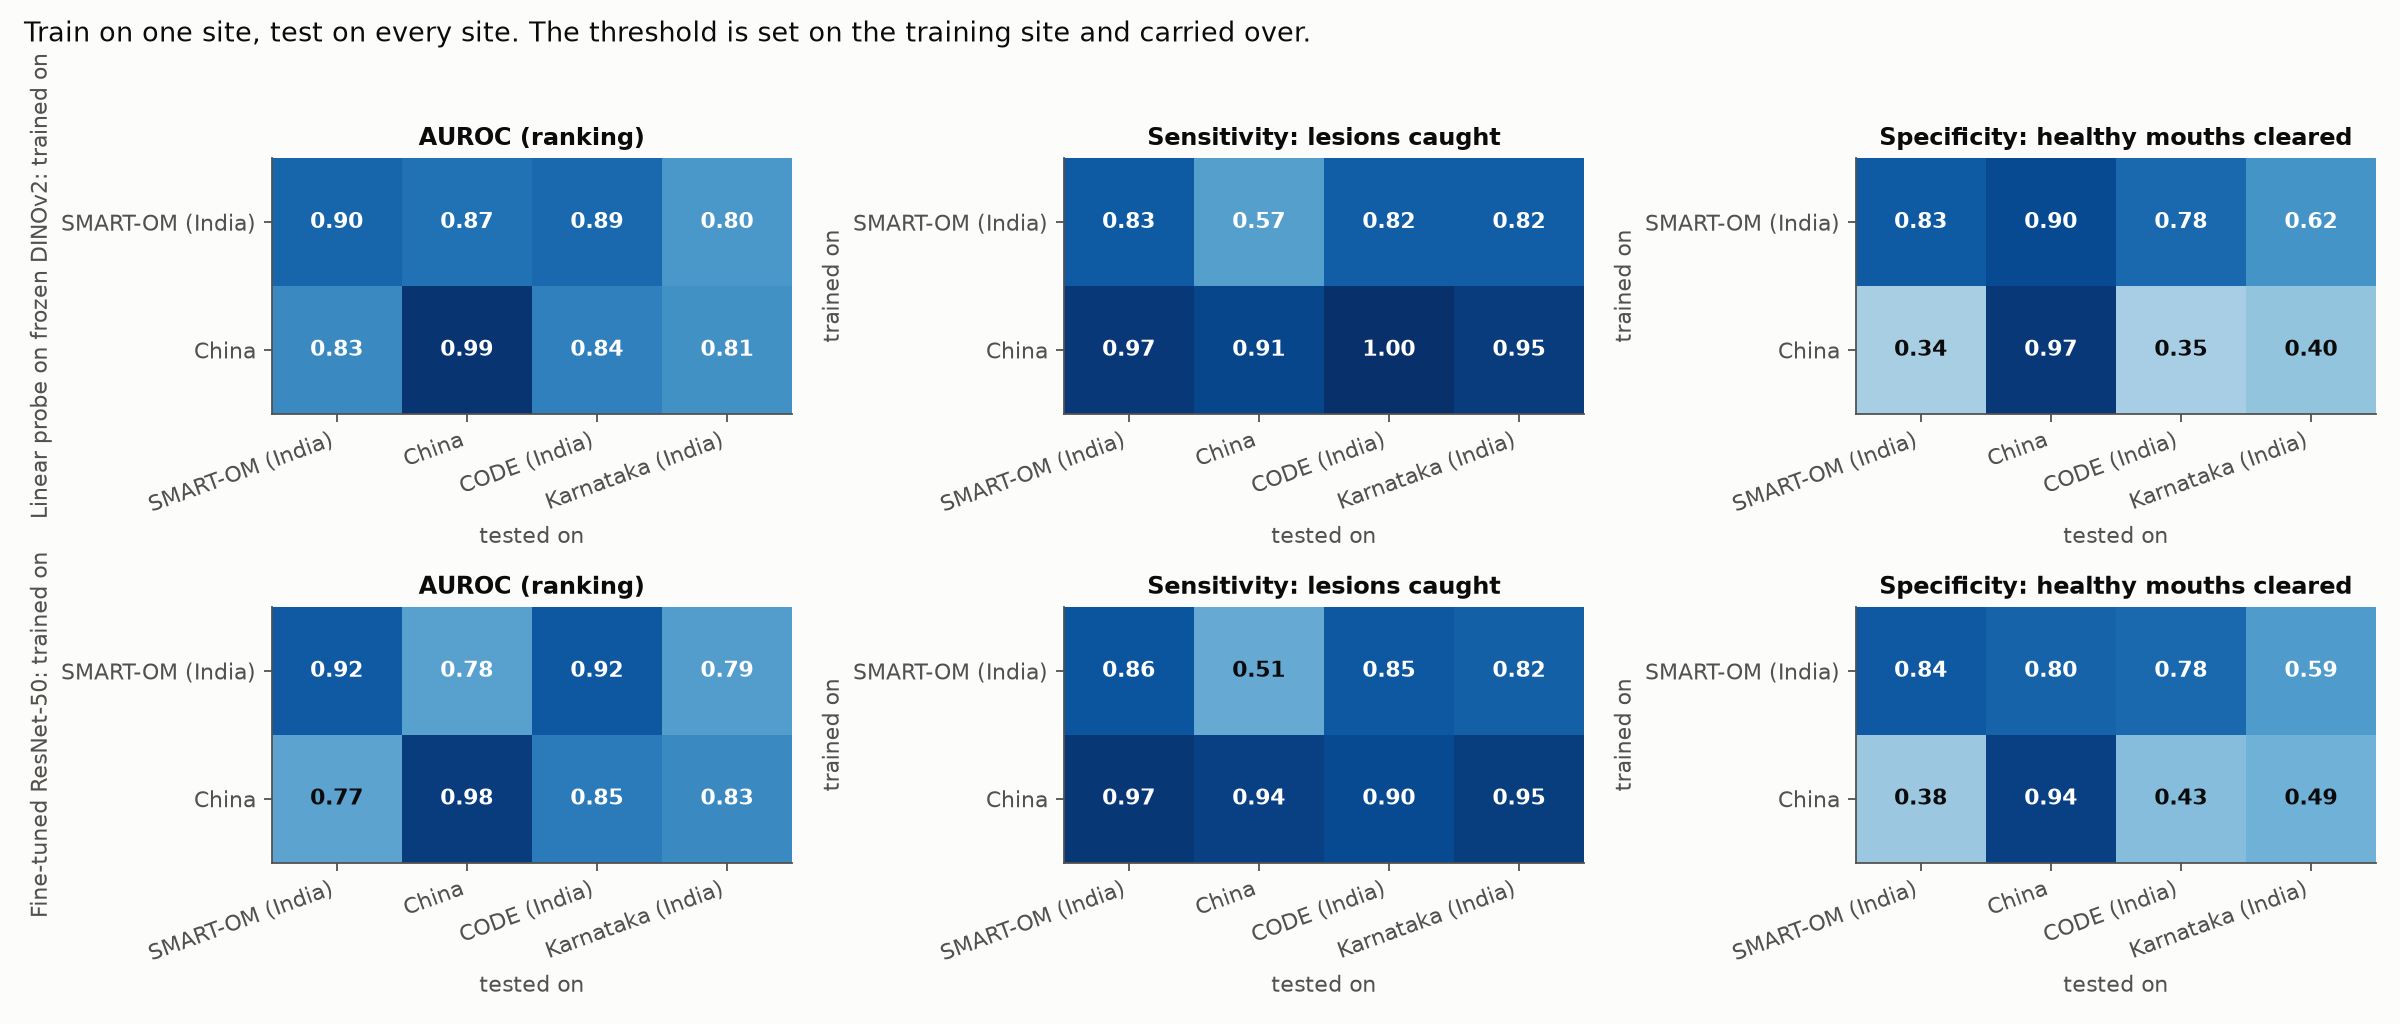
\includegraphics[width=\linewidth]{figures/e1_matrix.png}
\caption{AUROC, sensitivity and specificity for every training and test site. Rows of each panel are training sites; columns are test sites. Top: DINOv2 probe. Bottom: fine-tuned ResNet-50.}
\label{fig:matrix}
\end{figure}

The two model families are close in-site. Between countries the fine-tuned ResNet loses more than the frozen probe: AUROC 0.78 against 0.87 from SMART-OM to China, and 0.77 against 0.83 from China to SMART-OM.

The move from SMART-OM to CODE, which share a research network and a written photo protocol, costs nothing for either model. CODE has only 13 refer photographs, so its sensitivity intervals are wide, but specificity there rests on 5{,}554 healthy photographs and is tightly estimated at 0.78, the same as in-site.

\subsection{Fixes}

Table~\ref{tab:fixes} and Figure~\ref{fig:fixes} compare models at sites they never saw. Colour augmentation changed AUROC by 0.00 to 0.03. With one training site, the frozen probe transferred better between countries than the fine-tuned ResNet, by 0.06 and 0.09. Training on both sites did not help the probe, which lost 0.03 on Karnataka. The colour-augmented ResNet trained on both sites gave the best result at both unseen sites: AUROC 0.96 (0.94--0.98) on CODE, with sensitivity 0.87 and specificity 0.89, and 0.83 (0.79--0.87) on Karnataka. On Karnataka its threshold still failed, with specificity 0.40 (0.32--0.47) against sensitivity 0.95. Because CODE shares a research network with SMART-OM, Karnataka is the cleaner test of a new site.

\begin{table}[t]
\centering
\caption{AUROC at sites the model never saw. Single-site rows average over the available training sites. Blank cells: a model trained on both sites has seen that site.}
\label{tab:fixes}
\small
\begin{tabular}{lcccc}
\toprule
Method & SMART-OM & China & CODE & Karnataka \\
\midrule
ResNet-50, one site & 0.77 & 0.78 & 0.89 & 0.81 \\
ResNet-50 + colour augmentation, one site & 0.80 & 0.78 & 0.90 & 0.82 \\
DINOv2 probe, one site & 0.83 & 0.87 & 0.87 & 0.81 \\
ResNet-50 + colour augmentation, both sites & & & 0.96 & 0.83 \\
DINOv2 probe, both sites & & & 0.87 & 0.78 \\
\bottomrule
\end{tabular}
\end{table}

\begin{figure}[t]
\centering
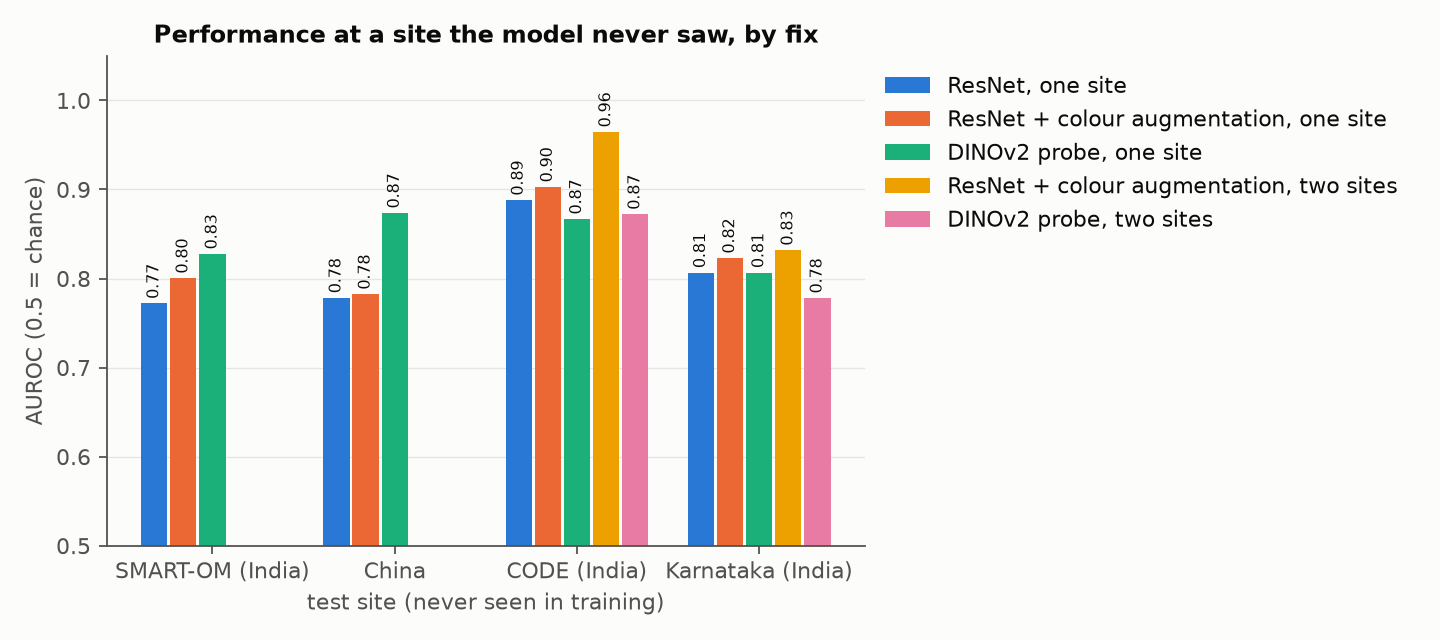
\includegraphics[width=0.85\linewidth]{figures/e2_fixes.png}
\caption{AUROC at unseen test sites for each method.}
\label{fig:fixes}
\end{figure}

\subsection{The conformal guarantee fails, and recalibration has a price}

Table~\ref{tab:conformal} and Figure~\ref{fig:conformal} report coverage and the share of photographs answered. In-site, coverage is 0.89 to 0.94 for both models, as promised. Moved to another research group's dataset, coverage falls to between 0.07 and 0.67, while the rule still answers 82\% to 93\% of photographs. Among the photographs it answers there, it is wrong 25\% to 92\% of the time for the probe.

With 50 labelled photographs from the new site the coverage promise holds again at every site, for both models. The recalibrated rule then answers 8\% to 46\% of photographs outside the SMART-OM network: it is honest, but mostly abstains. Figure~\ref{fig:conformal} (right) shows why: in-site, error falls as confidence rises; at a new site, error is high at every confidence level, and for the China-trained probe the most confident answers are the least accurate.

\begin{table}[t]
\centering
\caption{Conformal refusal at $\alpha = 0.1$. Each cell is coverage / share of photographs answered. Columns give the number of labelled test-site photographs used to recalibrate (0 = calibrated on the training site).}
\label{tab:conformal}
\footnotesize
\setlength{\tabcolsep}{4pt}
\begin{tabular}{llllll}
\toprule
Model & Train $\rightarrow$ test & 0 & 25 & 50 & 100 \\
\midrule
\multirow{8}{*}{DINOv2 probe}
 & SMART-OM $\rightarrow$ SMART-OM & 0.89 / 95\% & 0.94 / 83\% & 0.91 / 93\% & 0.89 / 94\% \\
 & SMART-OM $\rightarrow$ CODE & 0.88 / 94\% & 0.94 / 86\% & 0.90 / 92\% & 0.91 / 94\% \\
 & SMART-OM $\rightarrow$ China & 0.40 / 89\% & 0.96 / 14\% & 0.91 / 23\% & 0.91 / 25\% \\
 & SMART-OM $\rightarrow$ Karnataka & 0.67 / 89\% & 0.95 / 28\% & 0.93 / 41\% & 0.91 / 48\% \\
 & China $\rightarrow$ China & 0.92 / 93\% & 0.97 / 89\% & 0.92 / 93\% & 0.91 / 92\% \\
 & China $\rightarrow$ SMART-OM & 0.14 / 83\% & 0.98 / 3\% & 0.92 / 10\% & 0.91 / 12\% \\
 & China $\rightarrow$ CODE & 0.07 / 82\% & 0.95 / 6\% & 0.92 / 8\% & 0.92 / 8\% \\
 & China $\rightarrow$ Karnataka & 0.54 / 90\% & 0.97 / 14\% & 0.93 / 30\% & 0.92 / 34\% \\
\midrule
\multirow{8}{*}{\shortstack[l]{ResNet-50\\+ colour}}
 & SMART-OM $\rightarrow$ SMART-OM & 0.89 / 95\% & 0.93 / 81\% & 0.90 / 91\% & 0.89 / 94\% \\
 & SMART-OM $\rightarrow$ CODE & 0.89 / 95\% & 0.94 / 83\% & 0.91 / 93\% & 0.91 / 95\% \\
 & SMART-OM $\rightarrow$ China & 0.30 / 90\% & 0.97 / 9\% & 0.92 / 19\% & 0.92 / 19\% \\
 & SMART-OM $\rightarrow$ Karnataka & 0.65 / 89\% & 0.96 / 28\% & 0.92 / 46\% & 0.92 / 49\% \\
 & China $\rightarrow$ China & 0.94 / 98\% & 0.97 / 77\% & 0.92 / 94\% & 0.91 / 94\% \\
 & China $\rightarrow$ SMART-OM & 0.34 / 89\% & 0.94 / 10\% & 0.92 / 13\% & 0.91 / 16\% \\
 & China $\rightarrow$ CODE & 0.34 / 89\% & 0.94 / 9\% & 0.91 / 15\% & 0.91 / 14\% \\
 & China $\rightarrow$ Karnataka & 0.65 / 93\% & 0.96 / 23\% & 0.92 / 42\% & 0.91 / 43\% \\
\bottomrule
\end{tabular}
\end{table}

\begin{figure}[t]
\centering
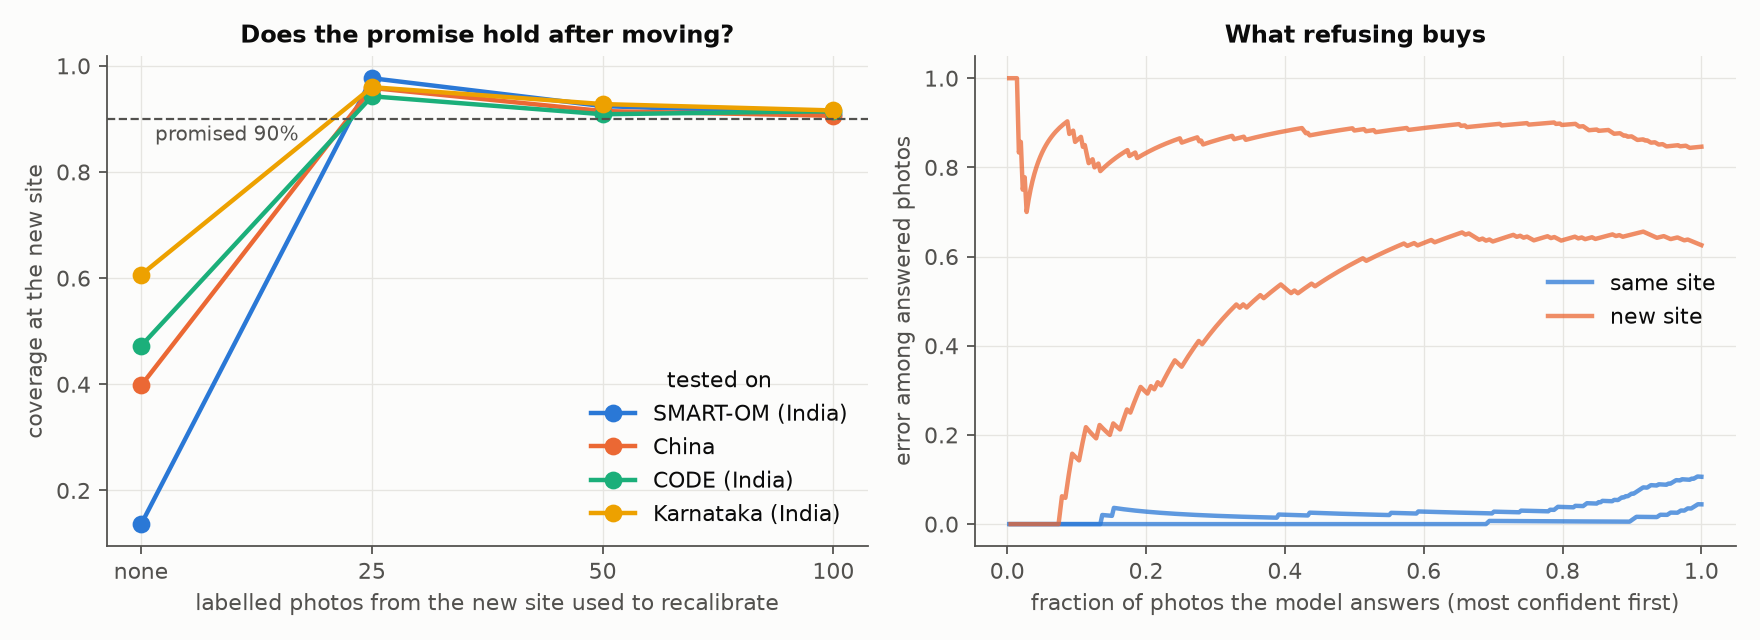
\includegraphics[width=\linewidth]{figures/e3_refusal.png}
\caption{Left: coverage of the DINOv2 probe at new sites against the number of labelled local photographs used to recalibrate; the dashed line is the promised 90\%. Right: error among answered photographs as the model answers more of them, most confident first, in-site (blue) and at new sites (orange).}
\label{fig:conformal}
\end{figure}

Even in-site the guarantee is marginal, not per class. Because healthy photographs dominate SMART-OM, the rule meets 90\% coverage overall while confidently clearing 33\% of SMART-OM's refer photographs.

\subsection{Healthy photographs reveal their dataset}

A linear classifier on frozen features told healthy photographs from two datasets apart with balanced accuracy 0.99 (China vs SMART-OM), 0.99 (China vs CODE), 0.96 (China vs Karnataka), 0.92 (CODE vs Karnataka), 0.91 (Karnataka vs SMART-OM) and 0.91 (CODE vs SMART-OM). Every dataset has a signature visible without any lesion.

\section{Discussion}
\label{sec:discussion}

\paragraph{A likely mechanism.} The share of refer photographs is 79\% in the China dataset and 6\% in SMART-OM, and every dataset can be recognised from healthy photographs alone. A model rewarded for predicting the label at home can therefore lower its loss by learning what a photograph from that dataset looks like, a shortcut in the sense of \citet{geirhos2020shortcut} and the same pattern \citet{zech2018variable} found across hospitals. The China-trained model's behaviour fits this account: it scores healthy Indian mouths at 0.84 on average, close to its home average for lesions. A signature alone is not enough to break a model. CODE and SMART-OM are separable at 0.91 and a model moved between them loses nothing; there the two datasets also share a photo protocol and a low prevalence of lesions, so the signature does not line up with the label. We have not isolated the mechanism, and a study that matched prevalence across sites, or removed the signature with domain-adversarial training \citep{ganin2016dann}, would test it directly.

\paragraph{What a reported in-site accuracy means.} AUROC fell modestly, by 0.03 to 0.21, and a reader who sees only AUROC could conclude that these models transfer reasonably. The quantities a screening programme acts on, the share of lesions referred and the share of healthy people sent home, moved by up to 63 percentage points. Studies of oral screening models should report sensitivity and specificity at a fixed, pre-registered threshold on an external dataset, not AUROC alone.

\paragraph{What fixes did.} Colour augmentation helped little, which argues against camera colour as the main cause. Fine-tuning all weights fitted each site more closely and transferred worse than a frozen feature extractor. The fine-tuned model trained on two sites was the only configuration that improved unseen-site AUROC, which is consistent with \citet{gulrajani2021lost}: variety in training data mattered more than the method. It did not fix the threshold on Karnataka.

\paragraph{A practical check for clinics.} Split conformal prediction assumes the calibration and test photographs are exchangeable, and a new site breaks that assumption \citep{tibshirani2019covariate}. Its failure here is silent: the rule kept answering most photographs while missing its target by up to 83 points. Fifty labelled local photographs restored the promise. A clinic considering such a tool could label 50 of its own photographs and look at how many the recalibrated rule still answers; for most moves we tested, the answer would show the tool is not usable there. A class-conditional version \citep{sadinle2019least} would also stop the guarantee from being met mainly on healthy photographs.

\paragraph{Datasets.} Two pairs of public datasets share photographs. Any study that trains on one member of a pair and tests on the other is partly testing on its training data, and the China and Karnataka copies disagree on the diagnosis. We recommend that oral photograph datasets publish file hashes and provenance, and that users check for overlap before cross-dataset evaluation.

\section{Limitations}

There are two training sites, which differ in country, phones and case mix at once; this study cannot separate those factors. A third training site, such as the Sri Lankan dataset of \citet{piyarathne2024dataset}, would allow a leave-one-site-out design. The SMART-OM test split has about 21 refer photographs and CODE has 13, so sensitivity on those sites is uncertain. China and Karnataka give no patient identifiers, and hash grouping catches re-saved copies but not two different photographs of one person. Part of the China dataset was collected from published literature, where lesions tend to be advanced, which may inflate its in-site scores. The ResNet models saw photographs resized to 320 pixels before the final 224-pixel resize, while the probe used full-resolution originals. Hyperparameters were fixed in advance and each configuration was trained once per seed. The diagnoses are those reported by the dataset owners. This is a retrospective study on public data, not a clinical evaluation.

\section{Conclusion}

On four public oral photograph datasets, classifiers that rank photographs well at home kept much of that ranking at a new site but lost their operating point and their conformal guarantee, and did so without signalling it. The datasets carry visible signatures and very different shares of lesions, which offers a likely shortcut. A small labelled sample from the new site is enough to detect the problem. External validation at a fixed threshold, and a check for shared images, should be routine in this area.

\section*{Reproducibility}

Code, the train/validation/test split of every photograph, saved predictions for every model and seed, and scripts that regenerate every table and figure are available at \url{https://github.com/sachchi-sapiens/oral-screen-shift}. The datasets are not redistributed; download scripts fetch them from their owners.

\bibliographystyle{plainnat}
\bibliography{references}

\end{document}
